\documentclass[letterpaper,12pt,twocolumn]{article}

\usepackage{amsmath,amssymb,mathpazo,xcolor,geometry,graphicx,multicol}
\geometry{top=0.75in,bottom=0.75in,right=0.75in,left=0.75in}
\graphicspath{../figures/}

\usepackage{biblatex}[backend=biber,citestyle=chicago-authordate]
\addbibresource{project2.bib}

\title{\Large Alternative Bandwidth Optimization Methods for Geographically Weighted Regression}
\author{Tyler D. Hoffman}
\date{3 December 2021}

\usepackage{hyperref}
\begin{document}
\maketitle

\section{Introduction}
\label{sec:introduction}
Geographically weighted regression (GWR; \cite{Fotheringham2003}) is a widely used statistical technique for analyzing spatial process variation and spatial relationships. The framework broadens a classical regression by allowing for spatially varying coefficients that illustrate different effects in different areas of the spatial domain. These coefficients are calibrated alongside a bandwidth parameter that controls the amount of spatial contextual information at a given location. During the fitting procedure, a local regression is fitted at every spatial observation using the information allotted by the bandwidth. Due to the influence it has on this process, the bandwidth parameter can be thought of as an indicator of the scale at which the process operates.

To find the bandwidth parameter, the fitting procedure makes use of a version of the Akaike information criterion (AIC; \cite{Akaike1973}) that incorporates a penalty term to disincentivize overly complex models. The GWR-corrected AIC, or AICc, takes the form \cite{Fotheringham2003} \begin{align*}
    \text{AICc} = -2\log f(y | \beta, \sigma^2, X) + \frac{2n(k+1)}{n-k-2}
\end{align*} where $f(y | \beta, \sigma^2, X)$ is the likelihood function for the model, $n$ is the number of observations (i.e., areal units), and $k$ is the effective number of parameters for the model. This paper regards the AICc as a function of the GWR bandwidth, which controls the amount of data used at a given observation to calibrate its local model. In GWR, the optimal bandwidth---the bandwidth that the model ultimately reports---is the one that minimizes the AICc.

Theoretically, this minimization problem is easy to frame. In practice, however, the computation can get messy. Since the AICc does not have an analytical derivative with respect to the bandwidth, the procedure must use a derivative-free optimization method to find its minimizer. As a consequence, the performance of this optimizer is severely constrained: no derivative information means that an optimization method must use heuristic or naive methods to find a minimum or learn the shape of the objective on its own. These handicaps can be costly in terms of performance and make it difficult to quickly and accurately solve the minimization problem.

Additional constraints or information about an optimization problem always help refine the optimization strategy. By exploiting elements of the problem's structure, it is possible to customize faster and more powerful optimization methods. Such information is even more important when the objective lacks a derivative, as the optimizers must make up for not knowing the slope of the function.

While many improvements have been made to GWR since its inception (in particular, the generalization of the method into MGWR \cite{Oshan2019}), this paper focuses on the original procedure for simplicity. Indeed, this paper aims to deconstruct the optimization procedure for the GWR bandwidth and to examine the interplay between the structure of the problem and solution methods. By analyzing the problem's structure, it is possible to extract more insights about viable research directions for more efficient and reliable optimization techniques.

\section{Problem Structure}
\label{sec:problem}
Following ideas developed in \cite{Hoffman2021}, it is natural to consider the AICc as a combination of two terms acting independently: the log-likelihood (as a proxy for model fit) and the GWR correction (as a penalty for overfitting). Both of these vary as a function of bandwidth, but the way in which they vary differs between the two. The GWR correction is a monotonically increasing function of $k$ and blows up at $k = n-2$ due to its denominator--- \begin{align*}
    \lim_{k\rightarrow n-2} \frac{2n(k+1)}{n-k-2} = \infty
\end{align*} ---but recovers ``normal'' behavior after moving beyond this asymptote. Recall that $k$ is the effective number of parameters for a particular bandwidth; that is, the number of independent coefficient estimates calibrated by the model. Thanks to the generality of GWR, the model reverts to a global model when the bandwidth is infinite---that is, when all the locations borrow data from each other, $k = p$ (the number of covariates at the global level). Conversely, when the bandwidth is 0, each location has a completely independent regression calibrated at it and therefore there are effectively $n$ independent parameters being calibrated. Hence, $k \in [p, n]$ is a decreasing function of bandwidth and the correction is a decreasing function of the bandwidth as well.

In fact, the GWR correction is a very well-behaved decreasing function of the bandwidth. The log-likelihood, on the other hand, evades such guarantees. As such, the log-likelihood drives the AICc curve; the strength of its counterbalance to the GWR correction is what determines where the optimal bandwidth lies.

Figure \ref{fig:sample-aicc} showcases a well-behaved AICc created from synthetic data. The curve has three attributes that may prove challenging for optimizers to handle: its minimizers, its steepness, and its noise. Each of these will be discussed in the following subsections.

\begin{figure}
    \centering
    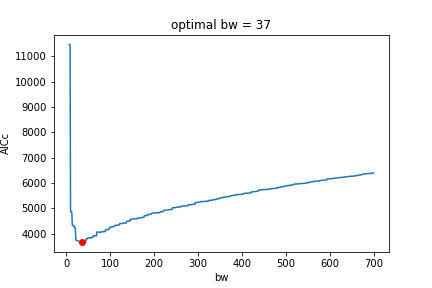
\includegraphics[width=0.5\textwidth]{../figures/sample-aicc.png} 
    \caption{An example of a well-behaved AICc curve with the absolute minimum marked in red.}
    \label{fig:sample-aicc}
\end{figure}

\subsection{Minima}
As discussed above, minimizers of an AICc curve indicate appropriate bandwidths for analysis and the absolute minimizer is the best bandwidth for analysis. If the absolute minimizer is on the boundary of the search domain, then the process is local (left boundary) or global (right boundary). Optimization methods, however, may run into issues if the AICc curve exhibits multiple minima. Local minima occur at bandwidths where model fit is markedly better than the bandwidths in the surrounding region, but does not outpace the complexity correction enough to dominate the absolute minimum. These can be thought of as artifacts of the modifiable areal unit problem (MAUP), although they can be difficult to distinguish from noise (Section \ref{sec:problem-noise}). Some optimizers are prone to getting trapped in local minima, so any optimization done on AICc curves must be robust to this. 

\subsection{Steepness}
Since the GWR correction is fixed and monotonic, the steepness of the curve is almost wholly determined by the log-likelihood. As remarked earlier, process variation plays a big role in influencing the shape of the AICc curve. Here, an interval where the curve is very flat indicates that the bandwidths in that interval would all be fairly viable. In cases when the process is global, the absolute minimum is on the right boundary of the search domain and the curve is often very flat near it. Due to the Extreme Value Theorem, the AICc (a continuous function of the bandwidth) is guaranteed to have a minimum so long as the search interval is closed and bounded. However, convergence to this minimum can be very slow when the curve is nearly flat, since the optimization methods are not privy to the slope of the function.

Moreover, the confidence in this minimum can be low even though the minimum is well-defined. Current GWR software allows for the computation of bandwidth confidence intervals, produced by randomizing the initialization for a golden-section search and performing inference on the resulting data. If the curve is essentially flat near the minimum, then golden-section search will often achieve its desired convergence tolerance long before attaining the minimum, thus leading to the aforementioned wide confidence intervals. In the limit, this distribution will concentrate around the absolute minimum, but the rate of this concentration may be slow. 

\subsection{Noise}
\label{sec:problem-noise}
Noise in the AICc curve is natural for real datasets due to the calibration process. If some areal units are much larger than others, then the model fit might drastically change when the bandwidth becomes large enough to borrow data from those locations. In this way, the AICc curve may become sensitive to small perturbations in the bandwidth and develop jagged-looking noise. These jitters in the AICc curve are not meaningful local minima, but it could be difficult for an optimization algorithm to determine that. In short, any viable optimizer must be able to distinguish between noise, a local minimum, and the absolute minimum.

\section{Methods}
\label{sec:methods}
\subsection{Optimizers}
This work tests four optimizers for finding the optimal bandwidth. First, grid search (brute force optimization) is presented as a baseline for performance benchmarking. Next, a version of golden-section search \cite{Kiefer1953} similar to the implementation in the Python \texttt{mgwr} module was tested \cite{Oshan2019}. Golden-section search looks for the minimum of a unimodal function in a specified interval by repeatedly bisecting that interval according to the golden ratio ($\phi = (1 + \sqrt{5})/2$). By enforcing this proportion, the search algorithm offers a good rate of convergence to the minimum without sacrificing much in the way of accuracy. However, when applied to multimodal functions such as the AICc curve, golden-section search is known to get trapped in local minima. One proposal to avoid this is to use different initial points for golden-section search and to use the best result. More research is required to determine what guarantees this lends to the search method.

Another prototypical derivative-free optimizer, Brent's method, was also tested \cite{Brent1973}. Brent's method combines the bisection method and a quadratic version of the secant method (inverse quadratic interpolation instead of linear interpolation) by testing how much each method improved the solution at each iteration. By balancing the two, it has a worse worst-case complexity than the bisection method, but converges superlinearly if the objective is well-behaved.

Finally, particle swarm optimization (PSO) was considered as a heuristic approach to optimization \cite{Bonyadi2017}. PSO lets loose a swarm of particles (candidate solutions) in the domain which search for minima by moving with a certain amount of velocity. On each iteration, the particles use this built-in velocity, knowledge of their own best position, and knowledge of the swarm's best position to determine where to move. As a result, PSO can effectively explore local minima: as long as one particle reaches the absolute minimum, the swarm has succeeded. Additionally, due to the highly parallel behavior of the particles, PSO lends itself well to parallel computing implementations. These can improve the runtime of the algorithm, but do not improve the number of objective calls done by the algorithm. While these parallel methods are not explored in this paper, they could offer significant practical speedups in implementation.

All the optimizers were run with a tolerance of $\varepsilon = 10^{-10}$ and up to a maximum number of iterations of 1000. PSO used a fixed inertia weight of -0.16, a cognitive coefficient of 1.89 (weight given to the particle's own history), and a social coefficient of 2.12 (weight given to information from the rest of the swarm). These values were heuristically tuned through observation and informed by the literature \cite{Bonyadi2017}.

\subsection{Sample Data}
As explained in Section \ref{sec:problem}, the AICc curves typically look like smooth checkmarks. The baseline curve (Figure \ref{fig:baseline}) was therefore chosen to be $b(x) = (x^2 - x + 600)/2x$ for $x > 0$ as it depicts well this smooth, unimodal shape. Subsequently, this objective was altered along the three axes of study: minima, steepness, and noise. All experiments were conducted with a low amount of added noise to simulate how real AICc curves behave.

To introduce multiple minima, a rule was prescribed that adds more checkmark-shaped curves along fixed displacements (Figure \ref{fig:multiple-mins}). The extra checkmarks take the form \begin{align*}
    g(x) = 0.0005((x-120)/10)^8 + x - 65
\end{align*} and for a given set of new minima locations $\{a_i\}_{i=1}^m$ were displaced to create a set of functions \begin{align*}
    h_i(x) = g(x - a_i) + a_i/2, i = 1, \dots, m.
\end{align*} Finally, for each $x$, the multiple minimum objective was defined as \begin{align*}
    b_m(x) = \min \{b(x), h_1(x), \dots, h_m(x)\} + \text{noise}.
\end{align*} 

For steepness, the baseline curve was parametrized with an additional steepness factor that altered the slope of the curve's tail (Figure \ref{fig:steep-curves}). These curves took the form \begin{align*}
    b_\sigma(x) = (\sigma x^2 - x + 600)/2x + \text{noise}
\end{align*} where $\sigma > 0$ was the steepness parameter.

To add the noise, the generalized Hénon map was used \cite{Henon1976}. The noise needed to be non-random so it could be controlled across all optimizers, so a hyperchaotic dynamical system was utilized to ensure the noise could not be predicted but were replicable. The update rule for the discrete-time dynamical system takes the form \begin{align*}
    x_i = a - x_{i-1}^2 - bx_{i-2}
\end{align*} where $a = 1.76$ and $b = 0.1$ are taken to be fixed parameters that are known to generate hyperchaos. To generate the noise, the system was run for 100 iterations using initial conditions $x_0 = 0$ and $x_1 = x$, where $x$ is the point for which the noise was requested (Figure \ref{fig:noisy-curves}). The variance of the noise could then be adjusted simply by scaling the output from the Hénon map generator.

\begin{figure}
    \centering
    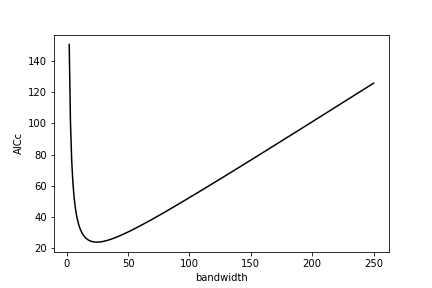
\includegraphics[width=0.5\textwidth]{../figures/baseline.png} 
    \caption{The base curve used for the numerical experiments.}
    \label{fig:baseline}
\end{figure}

\section{Results and Discussion}
\label{sec:results}
Figures \ref{fig:multmins-res}, \ref{fig:steep-res}, and \ref{fig:noisy-res} contain the results of the experiments. Each figure contains four performance metrics: the number of calls to the objective function, the absolute error between the result and the true minimum, the wall time, and the number of iterations to convergence. Among these, the number of function calls is the most useful metric as these are very computationally expensive---every function call requires a full GWR calibration. The number of function calls is also algorithm-dependent and architecture-independent. On the other hand, wall time refers to the total runtime of the algorithm based on a proverbial ``clock on the wall.'' This is not in general a good marker of performance since the total runtime can fluctuate based on implementation details and system architecture. Since these experiments are on sample curves with specified shapes, the function calls are each very computationally cheap because there is no GWR calibration associated with them, but the number of function calls is the same as if the curves were generated by fitting a GWR model at each bandwidth.

In each of the three experiments, grid search offers a baseline to compare against the rest of the methods. The best-case, worst-case, and average-case performance of grid search are all the same complexity, since the optimizer computes the function value at every requested location. Therefore, its number of function calls will always be 1000 (the maximum number of iterations) since that value does not change with the tolerance. Simultaneously, grid search performs well for all the curves, since it naively samples the entire function and returns the minimum it computed. As such, grid search is very computationally expensive, but often the best performing method despite this impracticality.

All of the optimizers considered in these experiments performed roughly the same regardless of the number of minima, except for PSO (which jumped around a common accuracy but was not exactly constant). This robustness indicates their viability as optimization methods for GWR, since they can easily handle curves with multiple local minima.

PSO has a hard time dealing with noise, but does not have the same issue with multiple minima. All of the experiments show evidence that the optimizer can be very efficient in terms of function calls, but needs tweaking for accuracy. While these experiments fixed the number of particles used in the optimization at 40, earlier experiments with fewer particles yielded less accurate results but better computational complexity. Hence, there is a tradeoff apparent in the number of particles. This, in combination with more extensive hyperparameter tuning, could be interesting future experiments in improving the efficacy of PSO. Since the AICc curves typically follow a similar shape, it is likely that there may be good-performing hyperparameter values that do not need to be tuned for the problem at hand.

A complexity-accuracy tradeoff appears between Brent's method and golden-section search. Across the experiments, Brent's method consistently required fewer function calls, but returned less accurate results. Even though both methods broke down as noise intensified, Brent's method still required fewer function calls than golden-section search. More exhaustive testing is required to examine this tradeoff, but these results suggest a useful niche for Brent's method for quick, back-of-the-napkin bandwidth optimizations.

\section{Conclusion}
\label{sec:conclusion}

This work is a conceptual deconstruction of the GWR-corrected AICc. It examines attributes of the AICc as a function of the bandwidth in pursuit of a well-designed optimization method that exploits knowledge of this problem's structure. Several of such optimizers were tested in a series of numerical experiments.

This study was limited in time and scope and would benefit from a more mathematical analysis of the internal mechanics of GWR. Recent analyses (\cite{Feng2021}'s deconstruction of stochastic gradient descent, e.g.) have conducted deep dives into existing methods that shed light on why the methods work. Importantly, the papers then extend these insights to develop novel improved variants. It would be interesting and possibly fruitful to follow a similar procedure for GWR.

Future work on this research direction would require more exhaustive experiments that dig into the interplay between the optimization methods and the three components of minima, steepness, and noise. Additionally, it would be important to address the broad variety of PSO variants and consider the implications of choosing different implementations. The metaoptimization of PSO hyperparameters was only cursorily considered in this work, and would be critical to examine further in order to determine the true viability of the method. Also, a detailed dive into local minima of the AICc curve is warranted---indeed, the idea of giving meaning to local minima at all may be faulty (everything but the absolute minimum might just be noise).

\subsection*{Code availability}
\href{https://github.com/thoffman1/gwr-optimizers}{This Github repository} contains the code used to run the experiments in this paper.

\printbibliography
\pagebreak

\onecolumn
\section*{Large Figures}
\label{sec:figs}

\begin{figure}[h!]
    \centering
    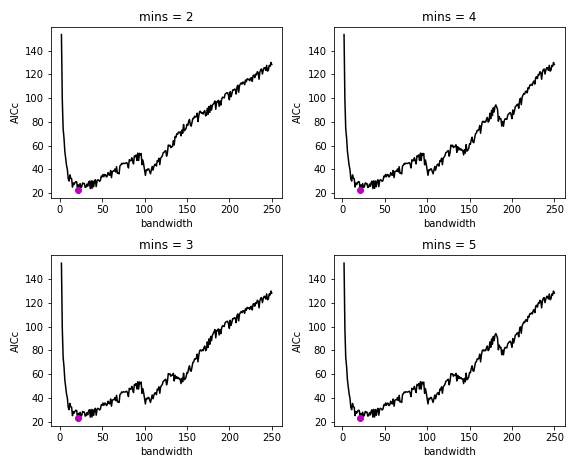
\includegraphics[width=\textwidth]{../figures/multiple-mins-curves.png}
    \caption{Examples of four numbers of minima used in the numerical experiments.}
    \label{fig:multiple-mins}
\end{figure}

\begin{figure}
    \centering
    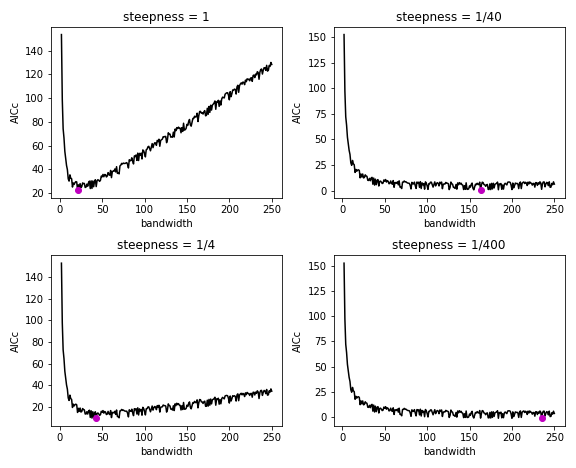
\includegraphics[width=\textwidth]{../figures/steep-curves.png}
    \caption{Examples of four steepness levels used in the numerical experiments.}
    \label{fig:steep-curves}
\end{figure}

\begin{figure}
    \centering
    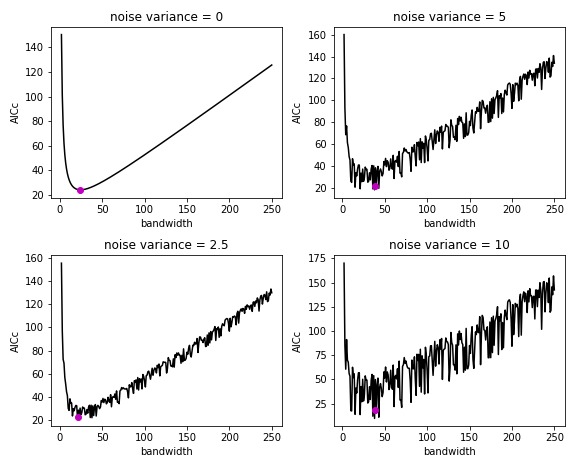
\includegraphics[width=\textwidth]{../figures/noisy-curves.png}
    \caption{Examples of four noise levels used in the numerical experiments.}
    \label{fig:noisy-curves}
\end{figure}

\begin{figure}
    \centering
    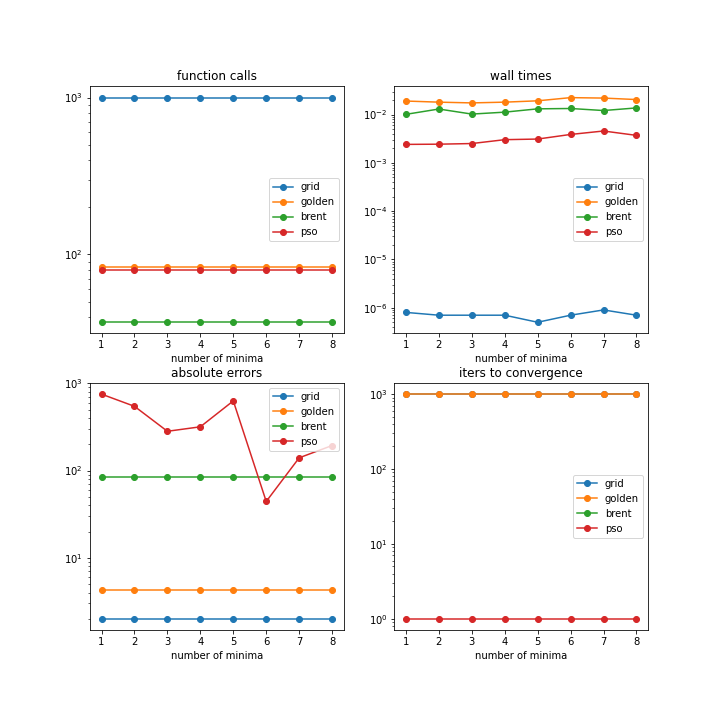
\includegraphics[width=\textwidth]{../figures/multmins-res.png}
    \caption{Results for testing the optimizers on curves with multiple minima. In this and the next two figures, the bottom left plot has grid search and Brent's method obscured by golden-section search.}
    \label{fig:multmins-res}
\end{figure}

\begin{figure}
    \centering
    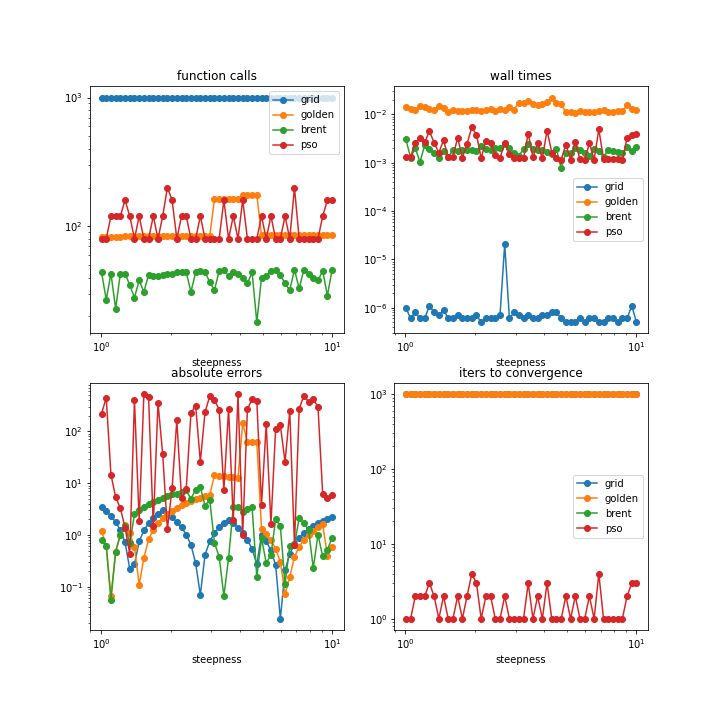
\includegraphics[width=\textwidth]{../figures/steepness-res.png}
    \caption{Results for testing the optimizers on curves with varying steepnesses.}
    \label{fig:steep-res}
\end{figure}

\begin{figure}
    \centering
    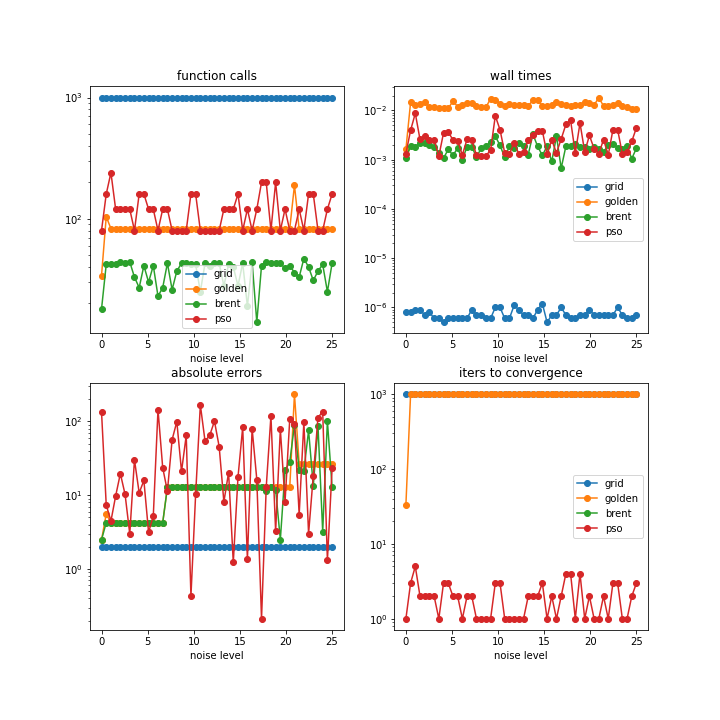
\includegraphics[width=\textwidth]{../figures/noisy-res.png}
    \caption{Results for testing the optimizers on curves with varying levels of noise. In the bottom left plot, the results for grid search are obscured by the Brent and golden-section search curves.}
    \label{fig:noisy-res}
\end{figure}

\end{document}